\section{Synteza dźwięku fletu}

W literaturze 

W niniejszym rozdziale przedstawiono dwa podejścia do implementacji syntezy dźwięku drewnianego instrumentu dętego:
\begin{itemize}
	\setlength\itemsep{-3pt}
	\item za pomocą falowodu cyfrowego,
	\item za pomocą zidentyfikowanego modelu ARMA fletu.
\end{itemize}


\subsection{Synteza falowodowa dźwięku fletu}
%https://ccrma.stanford.edu/~jos/pasp/Digital_Waveguide_Models.html
%https://quod.lib.umich.edu/cache//b/b/p/bbp2372.1992.072/bbp2372.1992.072.pdf#page=1;zoom=75
Synteza falowodowa instrumentów dętych drewnianych opiera się głównie na cyfrowych liniach opóźniających, które symulują odbicia fali w komorze dźwiękowej (ang. bore) tego rodzaju instrumentów.

\subsubsection{Model}
\begin{figure}[H]
	\centering
	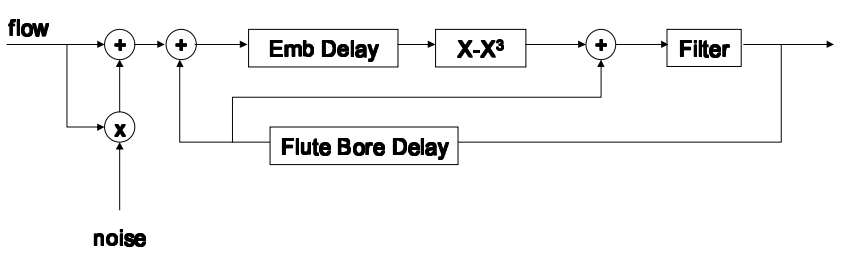
\includegraphics[width=12cm]{grafiki/flute_waveguide_mod}
	\captionsetup{justification=centering}
	\caption{Model falowodowy prostego instrumentu dętego drewnianego.}
	\label{rys:plaszcz_Z}
\end{figure}

\subsubsection{Implementacja}
W autorskim programie realizowanym na procesorze DSP implementację oparto na modelu falowodowym P. Cook'a.


\subsection{Synteza dźwięku fletu na podstawie modelu ARMA}
W tym podrozdziale przedstawiono znalezienie modelu fletu na podstawie manualnego doboru jego parametrów. Do identyfikacji instrumentu użyto dźwięku A razkreślnego o częstotliwości 440Hz. Dźwięk fletu zmienia swoją charakterystykę wraz z upływem czasu po chwili pobudzenia (dmuchnięcia w ustnik przez flecistę). Oznacza to, iż model zmienia się w trakcie przebiegu sygnału.

\subsubsection{Identyfikacja modelu}
Identyfikacja modelu matematycznego instrumentu została przeprowadzona dwoma sposobami: 
\begin{itemize}
	\item manualne dopasowanie zer i biegunów modelu, 
	\item użycie funkcji wbudowanej w środowisko symulacyjne Matlab.
\end{itemize}

Z uwagi na zmienność modelu fletu w czasie, ze zpróbkowanego sygnału wybrano 4096 próbek z miejsca w czasie, w którym sygnał miał stosunkowo stałą charakterystykę. Na tym fragmencie sygnału przeprowadzono dyskretną transformatę Fouriera za pomocą algorytmu FFT.


Na wykresie przedstawiającym widmo częstotliwościowe można zauważyć wyraźne piki oraz doliny charakterystyki. Następnym krokiem w przeprowadzanej identyfikacji było określenie częstotliwości oraz amplitud widocznych pików oraz dolin. Siedem pierwszych pików charakterystyki zostało zinterpretowanych jako bieguny modelu, natomiast sześć pierwszych dolin charakterystyki częstotliwościowej zamieniona została na zera modelu. Liczba wybranych pików i dolin wziętych pod uwagę przy tworzeniu modelu, została dobrana na podstawie wzrokowej oceny ilości harmonicznych mogących mieć znaczny wpływ na ukształtowanie brzmienia zsyntezowanego instrumentu. Częstotliwości rezonansowe przetworzono według zależności:
\begin{equation} \label{equ:wzor3}
p = 1-\frac{0.05}{A_{p}}e^{jf_{p}2\pi/F_{s}}
\end{equation}
\begin{equation} \label{equ:wzor4}
q = 1-\frac{0.05}{A_{q}}e^{jf_{q}2\pi/F_{s}}
\end{equation}
\begin{tabular}{ l l l l}
	gdzie: & $p$ &  - & bieguny modelu, \\
	&	$q$ & - &  zera modelu, \\
	&	$F_{s}$ & - &  częstotliwość próbkowania nagranego dźwięku,\\
	&	$f_{p,q}$ & - &  częstotliwość rezonansowa biegunów i zer modelu, \\
	&	$A_{p,q}$ & - &  amplituda rezonansu zer i biegunów, \\
\end{tabular} 
\vspace{6pt}

Każdy pik został przetworzony na dwa bieguny odbite lustrzanie względem osi realis na płaszczyźnie Z, natomiast każda dolina została przetworzona na dwa zera odbite lustrzanie względem osi Z.
\begin{figure}[H]
	\centering
	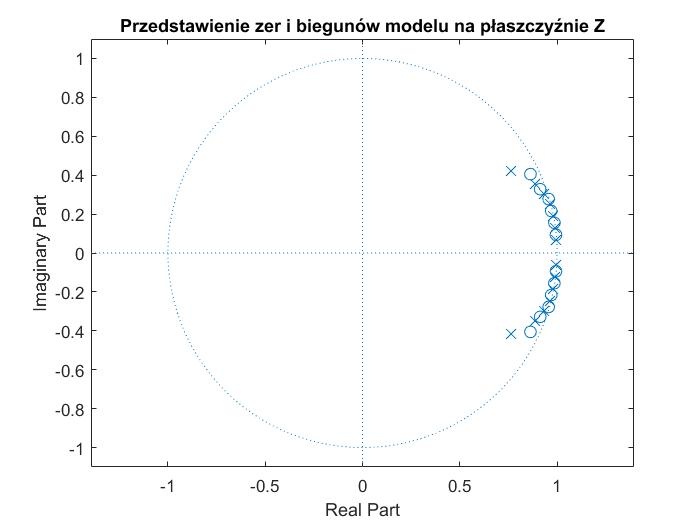
\includegraphics[width=6.5cm]{grafiki/Bieguny_na_plaszcz_Z}
	\captionsetup{justification=centering}
	\caption{Przedstawienie biegunów i zer modelu na płaszczyźnie Z.}
	\label{rys:plaszcz_Z}
\end{figure}
Model ARMA zsyntezowanego fletu utworzono na podstawie wyznaczonych zer i biegunów widocznych \ref{rys:plaszcz_Z}. W celu wydobycia dźwięku z modelu, pobudzono go sygnałem szumu białego, a następnie znormalizowano w celu uniknięciu przesterowania sygnału. 


Wydobyty dźwięk z modelu przypomina brzmienie instrumentu z rodziny instrumentów dętych drewnianych. Wysokość dźwięku wydobytego tonu jest taka sama jak oryginalnego dźwięku (440Hz).

\subsubsection{Parametryzacja zidentyfikowanego modelu}
Gra na instrumencie wymaga wydobywania z niego dźwięków o różnej wysokości. Zidentyfikowany w poprzednim punkcie model jest statyczny. Po pobudzeniu modelu szumem, wydobywa się z niego zawsze ten sam dźwięk (dźwięk A razkreślny, na podstawie którego, model był identyfikowany). W celu wydobycia innego dźwięku na podstawie utworzonego modelu, należy dokonać jego parametryzacji. Parametryzacja zidentyfikowanego modelu polega na uzależnieniu każdego biegunu i zera modelu od zagranego tonu.


Parametryzacja modelu opierać się będzie o zasady przyjęte w protokole MIDI. W protokole tym, każda wysokość dźwięku ma przypisaną liczbę od 1 do 127. Różnica między kolejnymi liczbami oznacza różnicę półtonu pomiędzy kolejnymi dźwiękami. Przykładowo dźwięk A razkreślny (o częstotliwości 440Hz) ma przypisaną liczbę 69, natomiast dźwięk B razkreślny (częstotliwość 466,2Hz) ma przypisaną liczbę 70. Między tymi dźwiękami występuje różnica jednegu półtonu. Każdy kolejny półton jest częstotliwością poprzedniego przemnożoną przez pierwiastek dwunastego stopnia z dwóch.


Na podstawie wymienionych zależności, każdy biegun został uzależniony od częstotliwości podstawowej zidentyfikowanego modelu (440Hz). Częstotliwość podstawowa wymnożona przez pierwiastek dwunastego stopnia podniesiony do potęgi różnicy półtonów między częstotliwością 440Hz a częstotliwością pożądanego dźwięku pozwoliła utworzyć biegun lub zero w odpowiednim miejscu.
\begin{figure}[H]
	\centering
	\includegraphics[width=12cm]{grafiki/Model_B_A}
	\label{rys:por_mod_flet}
	\captionsetup{justification=centering}
	\caption{Porownanie modeli fletu dla dzwieku B razkreślnego (wykres przesuniety w prawo) i A razkreślnego (wykres przesunięty w lewo)}
	\label{rys:por_mod_flet}
\end{figure}
Na rysunku \ref{rys:por_mod_flet} widać, iż wszystkie piki oraz doliny opisane zidentyfikowanym modelem przesuwają się w dziedzinie częstotliwości dla różnych tonów. Oznacza to, iż pobudzony model wyda dźwięk o różnej wysokości dla różnych parametrów wejściowych.
\subsection{Synteza dźwięku fletu na podstawie zidentyfikowanego modelu AR oraz ARMA}
W tym podrozdziale zsyntezowany dźwięk zostanie wytworzony na podstawie modelu znalezionego w sposób algorytmiczny. Poszukiwane będą modele w postaci AR oraz ARMA dla dźwięku fletu, a następnie porównane pod względem rzędu oraz brzmienia po ich pobudzeniu.


W celu znalezienia modelu AR zaimplementowano estymator Yula-Walkera, który opiera się na wyliczeniu autokorelacji sygnału identyfikowanego procesu \cite{Y_W}. Rezultatem takiej estymacji są współczynniki procesu AR. Rząd modelu potrzebny do odnalezienia odpowiednio brzmiącego zsyntezowanego fletu wyniósł 300.



W celu znalezienia modelu autoregresyjnego ze średnią ruchomą użyto gotowej funkcji "armax()" wbudowanej w środowisko symulacyjne Matlab. Funkcja "armax()" pobiera dwa argumenty - sygnał, którego model jest identyfikowany oraz rząd mianownika i licznika tego modelu \cite{armax}. Estymator ten wykorzystuje zapętloną metodę przewidywania błędu do wykrywania parametrów modelu ARMA. Rząd modelu ARMA, który dawał dobre rezultaty po pobudzeniu go szumem (brzmiał podobnie do pierwotnego sygnału fletu) wyniósł 100. Przy takim rzędzie wciąż można usłyszeć 'cyfrowość' sygnału. Sygnał zsyntezowanego fletu brzmiał bardzo dobrze przy pobudzeniu modelu o rzędzie 500.


\begin{figure}[H]
	\centering
	\includegraphics[width=12cm, height=5cm]{grafiki/Model_AR_300}
	\captionsetup{justification=centering}
	\caption{Porownanie widm częstotliwości zidentyfikowanych modeli fletu w postaci AR oraz ARMA. Od lewej: Oryginalne widmo sygnału, widmo sygnału zidentyfikowanego procesu AR rzędu 300, widmo sygnału zidentyfikowanego procesu ARMA rzędu 100}
	\label{rys:por_ar_arma}
\end{figure}
Na rysunku \ref{rys:por_ar_arma} dokonano porównania widm częstotliwościowych dla różnych rzędów zidentyfikowanych modeli AR i ARMA. Wrażenia słuchowe są lepsze dla modelu ARMA 100 rzędu niż modelu AR 300 rzędu.

\subsection{Wzbogacenie brzmienia zsyntezowanych instrumentów dętych}
W poprzednich podrozdziałach znaleziono model matematyczny fletu. Model pobudzany był szumem w celu wydobycia się z niego dźwięku. Uzyskany dźwięk może wydawać się ‘statyczny’. W celu przybliżenia go do prawdziwego brzmienia fletu można wykonać na sygnale kilka operacji, które pomogą go udynamicznić:
\begin{enumerate}
	\setlength\itemsep{-3pt}
	\item[--] dodanie obwiedni dźwięku,
	\item[--] dodanie efektu vibrato,
	\item[--] zmiana charakteru pobudzenia.
\end{enumerate}
W kolejnych podrozdziałach omówiona zostanie obwiednia dźwięku oraz vibrato. Zmiana rodzaju pobudzenia (np. rodzaj szumu pobudzającego model) jest bardzo skomplikowanym tematem, charakterystycznym dla każdego instrumentu. Przykładem może być zamodelowanie zmiany dmuchnięcia flecisty w ustnik \cite{gest_flute}.
\subsubsection{Obwiednia dźwięku}
W celu ustalenia obwiedni generowanego dźwięku stosuje się klasyczny model ADSR (Attack Delay Sustain Release) \cite{adsr}, który stosowany był już w pierwszych syntezatorach analogowych.
\begin{figure}[H]
	\centering
	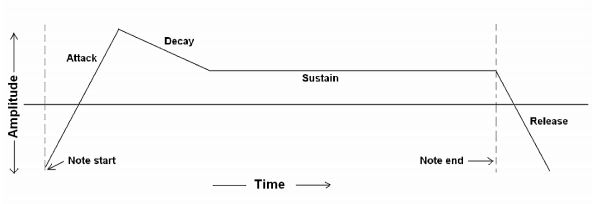
\includegraphics[width=9cm]{grafiki/ADSR}
	\captionsetup{justification=centering}
	\caption{Klasyczne podejście do obwiedni dźwięku.}
	\label{rys:adsr}
\end{figure}
Nałożenie obwiedni na zsyntezowany dźwięk pozwala na uzyskanie wyższej amplitudy w pierwszym momencie wydobycia dźwięku co przypomina moment dmuchnięcia flecisty w flet. Po chwili sygnał dźwięku jest bardziej statyczny co odpowiada podtrzymaniu dźwięku przez flecistę - "Sustain".
\begin{figure}[H]
	\centering
	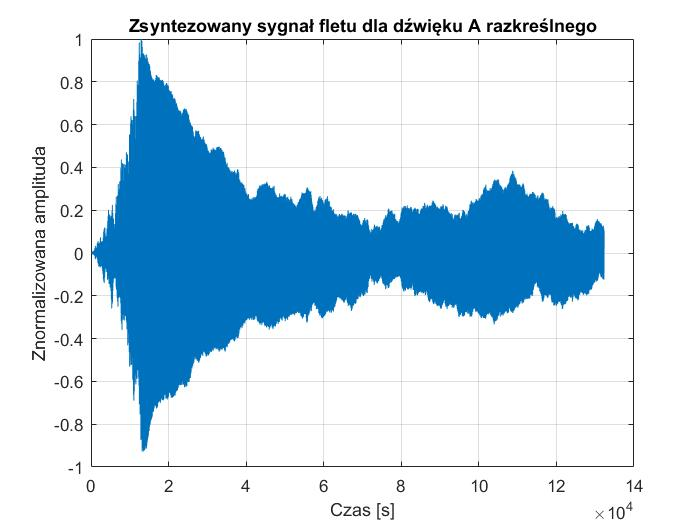
\includegraphics[width=9cm]{grafiki/Dzwiek_zsyntezowanego_fletu_po_ADSR}
	\captionsetup{justification=centering}
	\caption{Sygnał zsyntezowanego fletu po nałożeniu na niego obwiedni dźwięku}
	\label{rys:po_adsr}
\end{figure}
Na rysunku \ref{rys:po_adsr} można zauważyć wyraźny wpływ obwiedni dźwięku na wydobywany sygnał. Wrażenia słuchowe również wskazują na obecność wysokiej amplitudy sygnału na jego początku.

\subsubsection{Efekt vibrato}
W trakcie grania na wielu instrumentach rzeczywistych, aby urozmaicić wydobywany z instrumentu dźwięk, muzycy stosują technikę vibrato. W różnych rodzinach instrumentów efekt vibrato wydobywany jest w inny sposób. Na instrumentach smyczkowych lub strunowych powstaje on w wyniku delikatnego ruszania palcem na gryfie, natomiast w instrumentach dętych wydobywany jest już jako zaburzenie dmuchania flecisty w ustnik.


Z technicznego punktu widzenia efekt vibrato to delikatna modulacja częstotliwości podstawowej dźwięku, z niską częstotliwością drgań (wartość kilku lub kilkunastu Herzów). Wartość maksymalnej zmiany częstotliwości nie różni się zazwyczaj bardziej niż 1 procent wartości częstotliwości, wokół której oscyluje.


Implementację efektu vibrato przeprowadzono jako linię z opóźnieniem oraz efektem Doplera \cite{bowed_3}. Dodanie vibrato do dźwięku wydobywającego się z modelu spowodowało, iż brzmi on jest bardziej realistycznie.

\subsubsection{Implementacja}

\subsection{Interfejs użytkownika}